\section{Quantum Gates}

\begin{frame}{Qubits}
Qubit os a quantum system that exists in two possible states  $\ket{0}$ et $\ket{1}$. 
\newline \newline
A subit is a superposition, written as 
\begin{equation*}
    \ket{\Psi} = \alpha\ket{0}+\beta\ket{1}, \alpha \in \mathbb{C}, \beta \in \mathbb{C},  
    \textrm{ avec } |\alpha|^2+ |\beta|^2 = 1
\end{equation*}
for examle $\ket{\Psi} = 0.6\ket{0} + 0.8\ket{1}$ (et on a $0.6^2+0.8^2 = 0.36+0.64=1$)
\end{frame}

\begin{frame}{The Qubit Zoo}
Several kinds of physical qubits can de listed
\begin{itemize}
    \item spin of a particle(encoded on $\ket{UP}$ et $\ket{DOWN}$]
    \item excitation of an electron  (cold atoms, trapped ions=,  NV centers)
    \item supraconducting loops
    \item polarisation of a photon
    \item location of a particle in a system (toplogical qubit)
\end{itemize}
\end{frame}

\begin{frame}{Dirac's notation}
    Base quabits build the canonicam base for $\mathbb{C}^2$, in Direac's notation they are written as
\begin{equation*}
    \begin{split}
        \ket{0} &= \begin{pmatrix} 1 \\ 0 \end{pmatrix} \\
        \ket{1} &= \begin{pmatrix} 0 \\ 1 \end{pmatrix} \\
    \end{split}
\end{equation*}
Which eans that if $\ket{\Psi} = \alpha\ket{0}+\beta\ket{1}$
\begin{equation*}
    \ket{\Psi} = \begin{pmatrix} \alpha \\ \beta \end{pmatrix}
\end{equation*}
\end{frame}

\begin{frame}{One Qubit Gate}
All operator acting on qubits is unitary, which means
\begin{itemize}
    \item it's a matric in $\mathbb{C}^{2 \times 2}$, isomorphic to a  $4\times4$ real matrix, in
    $\mathbb{R}^4$
    \item as an unitary $U$, its  its adjoint matrix is the inverse of $U \times U^{\dag} = \mathbb{I}$ 
    \item it represent a rotation in $\mathbb{C}^2$ which can be seen as a rotation in $\mathbb{R}^4$
\end{itemize}
We have the operators $X$, $Y$ and $Z$
\begin{itemize}
    \item they are dual to Pauli operators from Quantum Physics
    \item they all "almost" dual to $i$, $j$ et $k$ from quaternions in $\mathbb{H}$
\end{itemize}
Every 1 qubit gate can be written as
\begin{equation*}
    U = a\mathbb{I} + bX + cY + dZ, a \in \mathbb{R}, b \in \mathbb{R}, c \in \mathbb{R}, d \in \mathbb{R}
\end{equation*}
\end{frame}

\begin{frame}{Superposition and H Gate}
The H gate, or \textit{Hadamard's gate} helps in building superposed states. \newline \newline
We have the following equations
\begin{equation}
\begin{split}
    H\ket{0} &= \frac{1}{\sqrt{2}}(\ket{0}+\ket{1}) = \ket{+}\\
    H\ket{1} &= \frac{1}{\sqrt{2}}(\ket{0}-\ket{1}) = \ket{-}
\end{split}
\end{equation}
H is a  $2\times 2$ matrix
\begin{equation*}
    H = \frac{1}{\sqrt{2}}\begin{pmatrix}
                           1 & 1 \\
                           1 & -1 \\
                          \end{pmatrix}
\end{equation*}
\end{frame}

\begin{frame}{X gate et qubit flips}
The X gate apparently works like the boolean NOT
\begin{equation*}
    X\ket{0} = \ket{1} \textrm{ et } X\ket{0} = \ket{1}
\end{equation*}
which means that
\begin{equation*}
    \textrm{If } \ket{\Psi} = \alpha\ket{0}+\beta\ket{1} \textrm{ Then } X\ket{\Psi} = \beta\ket{0}+\alpha\ket{1}
\end{equation*}
X is a $2\times 2$ matrix
\begin{equation*}
    X = \begin{pmatrix}
            0 & 1 \\
            1 & 0 \\
        \end{pmatrix}
\end{equation*}
It's important to realize that X is a rotation in $\mathbb{C}^2$ and no bollean operation. It's easy to build a square root 
of X, an "half X rotation" that you need to operate twice to have a complete X. 
Il est important de voir X comme une rotation et pas comme une inversion booléenne, on peut trouver une racine carrée
\begin{equation*}
     \sqrt{X} = \frac{1}{2}\begin{pmatrix} 1+i & 1 - i \\ 1 - i & 1 + i \end{pmatrix}  \textrm{ is such that }
     \sqrt{X}\times \sqrt{X} =  \begin{pmatrix} 0 & 1 \\ 1 & 0 \\ \end{pmatrix} = X
\end{equation*}
\end{frame}

\begin{frame}{Z gate and phase flip}
The Z gate reverses the phases, it reverse the sigh before the $\ket{1}$  component of a state \newline 
\begin{equation*}
    \textrm{Si } \ket{\Psi} = \alpha\ket{0}+\beta\ket{1} \textrm{ alors } Z\ket{\Psi} = \alpha\ket{0}-\beta\ket{1}
\end{equation*}
Z is a $2\times 2$ matrix
\begin{equation*}
 Z = \begin{pmatrix}
            1 & 0 \\
            0 & -1 \\
        \end{pmatrix}
\end{equation*}
The Y gate can be built using X and Z gates
\begin{equation*}
     Y = \begin{pmatrix}
            0 & -i \\
            i & 0  \\
        \end{pmatrix}  \textrm{ et } Y = iXZ
\end{equation*}
\end{frame}

\begin{frame}{This is an (electrical) circuit}
    \centering
    \includegraphics[width=10cm]{images/circuit_électrique.png}
\end{frame}

\begin{frame}{This is no pipe}
    \centering
    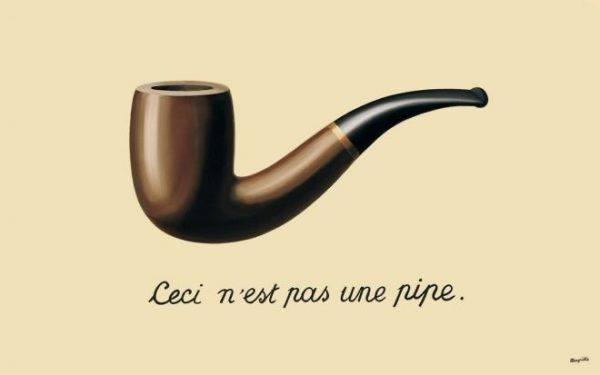
\includegraphics[width=10cm]{images/pipe.jpg}
\end{frame}

\begin{frame}{This is no circuit, this is actually a matrix!}
The following circuit build the famous \textit{EPR} pair
\begin{center}
\begin{tikzpicture}
    \node[scale=1.2] {
        \begin{quantikz}
           & \gate{H} & \ctrl{1} & \qw  & \qw \\
           & \qw      & \targ{}  & \qw  & \qw 
        \end{quantikz}
    };
\end{tikzpicture} 
\end{center}
This circuit is actually depicted by this matrix
\begin{equation*}
    \frac{1}{2}\begin{pmatrix}
                           1  &  0  &  1  &   0  \\
                           0  &  1  &  0  &   1  \\
                           0  &  1  &  0  &  -1  \\
                           1  &  0  &  -1 &   0  \\
                       \end{pmatrix}
\end{equation*}
\end{frame}


\begin{frame}{My first quantum circuit}
Gate based quantum programming builds complex matrices from simpler components.
\begin{center}
 \begin{quantikz}
       \qw  & \gate{H} & \gate{Z} & \gate{H} & \qw
\end{quantikz}
\end{center}
means: apply H, then Z, then H, which in gloabl apply the matrix product $H\times Z \times H$
\begin{equation*}
\begin{split}
    H\times Z \times H &= \frac{1}{\sqrt{2}}\begin{pmatrix}
                           1 & 1 \\
                           1 & -1 \\
                          \end{pmatrix} \times
                           Z = \begin{pmatrix}
                            1 & 0 \\
                            0 & -1 \\
                          \end{pmatrix} \times
                          \frac{1}{\sqrt{2}}\begin{pmatrix}
                           1 & 1 \\
                           1 & -1 \\
                          \end{pmatrix} \\
                        &= \frac{1}{2}\begin{pmatrix}
                                0 & 2 \\
                                2 & 0 \\ 
                        \end{pmatrix} = 
                        \begin{pmatrix}
                            0 & 1 \\
                            1 & 0 \\
                        \end{pmatrix} = X
\end{split}
\end{equation*}
THis shows that this circuit is equivalent to an X gate. 
\begin{center}
 \begin{quantikz}
       \qw  & \gate{H} & \gate{Z} & \gate{H} & \qw  & \textrm{ correspond à   } & \gate{X} & \qw
\end{quantikz}
\end{center}
\textbf{IMPORTANT~:}~Quantum circuit are a smart way of depicting a potentially huge (and unreadable) matrix. They are 
definitely no relatio with circuits involved in electronics. 

\end{frame}

\begin{frame}{Entanglement and CNOT gate 1/2}
The CNOT gate, or CX, intruduces entanglement. It introduces kind of "if-then-else" logic that leads to condutionnl 
statements\newline

CNOT acts on a 2 qubits state, if the first is $\ket{0}$, the second is untouched, but if it is $\ket{1}$, a X gate is 
applied on the second qubit.
\begin{equation*}
    CX\ket{00} = \ket{00}, CX\ket{01} = \ket{01}, CX\ket{10} = \ket{11}, CX\ket{11} = \ket{10}
\end{equation*}
CX is $4 \times 4$ matrix
\begin{equation*}
    CX = \begin{pmatrix} 1 & 0 & 0 & 0 \\ 0 & 1 & 0 & 0 \\ 0 & 0 & 0 & 1 \\ 0 & 0 & 1 & 0 \\ \end{pmatrix}
\end{equation*}
\end{frame}

\begin{frame}{Entanglement and CNOT gate 2/2}
Generically, if $x$ and $y$ are booleans  $(x,y) \in \{0,1\}^2$, then the first qubit $\ket{x}$  does not change while
 $\ket{y}$ becomes $\ket{x \oplus y}$ ($\oplus$ is the boolean XOR)
\begin{center}
    \begin{tikzpicture}
        \node[scale=1.0] {
            \begin{quantikz}
                \ket{x} & \qw & \ctrl{1} & \qw & \qw & \ket{x} \\
                \ket{y} & \qw & \targ{}  & \qw & \qw & \ket{x \oplus y}  
            \end{quantikz}
        };
    \end{tikzpicture}
\end{center}   
CX is a rotation in $\mathbb{C}^4$, isomorphic to a rotation in $\mathbb{R}^8$, we can do "half of it" and so compute a 
square root of CNOT
\begin{equation*}
\sqrt{CX} = \frac{1}{2}
            \begin{pmatrix}
                1 & 0 & 0 & 0 \\
                0 & 1 & 0 & 0 \\
                0 & 0 & 1+i & 1-i \\
                0 & 0 & 1-i & 1+i \\
            \end{pmatrix}   
\end{equation*}
\end{frame}

\begin{frame}{Building the EPR pair}
The EPR pair $\frac{1}{\sqrt{2}}(\ket{00}+\ket{11})$ is an entangled state built by this circuit
\begin{center}
        \begin{tikzpicture}
        \node[scale=1.0] {
            \begin{quantikz}
                & \ket{0} & \gate{H} & \ctrl{1} & \qw  & \qw \\
                & \ket{0} & \qw      & \targ{}  & \qw  & \qw 
            \end{quantikz}
        };
    \end{tikzpicture}
\end{center}
We can compute that
\begin{itemize}
    \item the H gate creates state  $\frac{1}{\sqrt{2}}(\ket{0}+\ket{1})\ket{0} = \frac{1}{\sqrt{2}}(\ket{00}+\ket{10})$
    \item on applique CX operate of each part of the sum and we get 
    $\frac{1}{\sqrt{2}}(CX\ket{00}+CX\ket{10}) = \frac{1}{\sqrt{2}}(\ket{00}+\ket{11})$
\end{itemize}

\end{frame}

\begin{frame}{Controlled gates}
CNOT gate is very important, we can used it to build any other controlled gate
\begin{itemize}
    \item knowing unitary operator $U$, it is applied on the second qubit if the first qubit is $\ket{1}$
    \item recursively, we can build double control... and more!
    \item knwoing square or forth root of $U$ is doable (it a rotation) and important in build $CU$ or $CCU$ gates
\end{itemize}   
\begin{center}
        \begin{tikzpicture}
        \node[scale=0.8] {
            \begin{quantikz}
                 &  \ctrl{1} & \qw  &  & &  \ctrl{2} & \qw    \\
                 &  \gate{U} & \qw  &  & &  \ctrl{1} & \qw    \\
                 &           &      &  &  & \gate{U} & \qw  
            \end{quantikz}
        };
    \end{tikzpicture}
\end{center}
The CCNOT gate, or Toffoli gate is well known
\begin{center}
    \begin{tikzpicture}
        \node[scale=0.8] {
            \begin{quantikz}
                \ket{x} & \qw & \ctrl{1} & \qw & \qw & \ket{x} \\
                \ket{y} & \qw & \ctrl{1} & \qw & \qw & \ket{y} \\
                \ket{z} & \qw & \targ{}  & \qw & \qw & \ket{z \oplus (x \land y)} 
            \end{quantikz}
        };
    \end{tikzpicture}
\end{center}
\end{frame}

\begin{frame}{Key ideas}
Quantum Programming is composing simple unitary operators as building blocks to build bigger and more complex operators
acting on $n$ qubits.
\begin{itemize}
    \item the \textbf{H gate or Hadamard gate} introduces one-qubit superposition
    \item the \textbf{porte X} or NOT gate looks like a boolean NOT but is actually a rotation (like all unitary operators) 
    \item the\textbf{CNOT gate} introduces quantum entanglement and helps building an "if-then-else" logic
\end{itemize}


Quantum Programming is
\begin{itemize}
    \item expressing a known problem as a unitary operator
    \item buold this unitary operator as a circuit
    \item benefit from acceleration (or lesser energy consumption) when executing the circuit
\end{itemize}
Most important: remmber that \textbf{all actions are ALWAYS unitary matrices}
\end{frame}
